\section{Methods}
\label{sec:methods}

The goal of our method is to generate a segmentation mask for an object of interest in each frame of a single image volume or video sequence using only point-wise annotations and without knowing the image type or object of interest beforehand.

To do so, we propose a novel approach within the Positive-Unlabeled learning setting, that learns the segmentation of the object identified by the point-wise annotations. Our method makes use of a non-negative risk estimator~\cite{kiryo17}, which heavily relies on knowing the proportion of positive samples in the data. While unavailable in our setting, we introduce a novel self-supervised method to estimate this key value via an iterative learning procedure within a Bayesian estimation framework. We then devise a stopping condition to halt training at an appropriate point. Last, a spatio-temporal tracking framework is applied to regularize the output of our approach over the complete volume information.

We describe our approach now in more detail. In the following subsection, we introduce the Positive-Unlabeled learning framework and its non-negative risk estimator. We then describe in 
Sec.~\ref{sec:pi_estim} our self-supervised approach to learn effective class priors. Last, we detail how we leverage the spatio-temporal regularizer, and provide our implementation details
in Sec.~\ref{sec:tracking} and Sec.~\ref{sec:implementation}, respectively.

\subsection{Non-negative Positive-Unlabeled learning}
\label{sec:nnpu}

We first briefly introduce and formulate Non-negative Positive-Unlabeled learning~\cite{kiryo17} in the context of semantic segmentation.

Traditional supervised learning, which we denote Positive/Negative learning (PN), looks to build a model \(f_{\theta}: I \mapsto [0;1]^{W \times H}\), where \(\theta\) is a set of model parameters, \(I\) is the input image with width $W$ and height $H$. Letting \(\bm{\mathcal{I}} = \{\mathcal{I}^i\}_{i=1}^{N}\) be the set of $N$ input images corresponding to an image volume or video sequence, 
each image $\mathcal{I}^i$ is composed of pixels, $\mathcal{X}^i=\mathcal{X}_p^i \cup \mathcal{X}_n^i$, where $\mathcal{X}_p^i$ and $\mathcal{X}_n^i$ denote the positive and negative pixels, respectively. We denote $\pi^i \in (0,1)$ as the proportion of positive pixels in image $i$, and $\bm{\pi} = \{\pi^i\}_{i=1}^{N}$ as the set of such proportions over all frames. 

Training $f$ to optimize $\theta$ can then be computed by minimizing the empirical risk of the form,
\begin{equation}
R_{pn}=\sum_{i=1}^{N} \left[ \frac{\pi^i}{|\mathcal{X}_p^i|}\sum_{x \in \mathcal{X}_p^i}\ell^+(f_{\theta}(x)) \right.+
\left. \frac{1-\pi^i}{|\mathcal{X}_n|} \sum_{x \in \mathcal{X}_n^i}\ell^-(f_{\theta}(x)) \right].
  \label{eq:pn}
\end{equation}
\noindent 
A popular choice for $\ell$ is the logistic loss, for which \(\ell^+(z)=\log(1+ e^{-z})\), \(\ell^-(z)=\log(1+e^{z})\) are the positive and negative entropy loss terms, respectively. In which case, Eq. \eqref{eq:pn} is the Balanced Cross-Entropy loss (BBCE).

Conversely, computing Eq.~\eqref{eq:pn} is infeasable in a PU settting, as neither $\bm{\pi}$ nor $\bm{\mathcal{X}}_{n}$ are known in advance. Instead, we have a set of unlabeled samples $\bm{\mathcal{X}}_{u}$ that contain both positives and negatives. As suggested in~\cite{duplessis15}, the negative risk (\ie the second term of Eq.~\eqref{eq:pn}) can however be re-written in terms of $\bm{\mathcal{X}}_{p}$ and $\bm{\mathcal{X}}_{u}$ as,

\begin{equation}
  \label{eq:nnpu}
R_{pu}=\sum_{i=1}^{N}\Biggl[ \frac{\pi^{i}}{|\mathcal{X}^{i}_{p}|}\sum_{x \in \mathcal{X}^{i}_p}\ell^+(f_{\theta}(x)) +
\Biggl( \frac{1}{|\mathcal{X}^{i}_{u}|}\sum_{x \in \mathcal{X}^{i}_u}\ell^-(f_{\theta}(x)) -
\frac{\pi^{i}}{|\mathcal{X}^{i}_{p}|}\sum_{x \in \mathcal{X}^{i}_p}\ell^-(f_{\theta}(x)) \Biggr) \Biggr].
\end{equation}

This is achieved by observing that $p(x) = \pi p(x|Y=1) + (1-\pi) p(x|Y=-1)$ and that the negative risk can be expressed as $ (1-\pi) \mathbb{E}_{X \sim p(x|Y=-1)}\left[\ell^-(f_\theta(X)) \right] =
\mathbb{E}_{X \sim p(x)}\left[\ell^-(f_\theta(X)) \right] - \pi \mathbb{E}_{X \sim p(x|Y=+1)}\left[\ell^-(f_\theta(X)) \right]$. In the case of expressive models such as Neural Networks, minimizing the objective of Eq.~\eqref{eq:nnpu} using stochastic gradient descent on mini-batches of samples tends to overfit to the training data, by driving the negative risk, (\ie the bottom term of Eq.~\eqref{eq:nnpu}) to be negative.

To circumvent this,~\cite{kiryo17} proposed to perform gradient ascent when the negative risk of a mini-batch is negative using the following negative risk,
\begin{equation}
  \label{eq:neg_risk}
R_{i}^{-}=\sum_{i=1}^N\Biggl(
 \frac{1}{|\mathcal{X}^{i}_{u}|}\sum_{x \in \mathcal{X}^{i}_u}\ell^-(f_{\theta}(x)) - 
\frac{\pi^{i}}{|\mathcal{X}^{i}_{p}|}\sum_{x \in \mathcal{X}^{i}_p}\ell^-(f_{\theta}(x)) \Biggr).
\end{equation}

Thus the complete training procedure for the PU setting with deep neural networks is described in Alg.~\ref{alg:sgdnnpu}. Specifically, when \(R_{i}^{-} < 0\), gradient ascent is performed by setting the gradient to \(-\nabla_\theta R_{i}^{-}\). 
%\algnewcommand\algorithmicforeach{\textbf{for each}}
%\algdef{S}[FOR]{ForEach}[1]{\algorithmicforeach\ #1\ \algorithmicdo}
\begin{algorithm}[H]
\caption{Non-negative PU learning}
\label{alg:sgdnnpu}
\begin{algorithmic}[1]
\Require{$f_\theta$: Prediction model \newline
  $\bm{\mathcal{I}}$: Set of images \newline
  $\bm{\mathcal{X}_p}, \bm{\mathcal{X}_u}$: Positive and unlabeled samples \newline
  $\bm{\pi}$: Set of class priors \newline
  $T$: Number of epochs}
\For{\texttt{epoch} $\gets 1$ to $T$}
\State Shuffle dataset into $N_{b}$ batches
    \For{$i \gets 1$ to $N_{b}$}
     \State Sample next batch to get $\mathcal{I}^i$, $\mathcal{X}_p^i$, $\mathcal{X}_u^i$, $\bm{\pi}^i$
	\State Forward pass $\mathcal{I}^i$ in $f_\theta$
	\State Compute risks as in Eq. \ref{eq:nnpu} and \ref{eq:neg_risk}
      \If{$R_{i}^{-} < 0$}
          \State Do gradient ascent along $\nabla_\theta R_{i}^{-}$
      \Else
          \State Do gradient descent along $\nabla_\theta R_{pu}$
      \EndIf
  \EndFor
\EndFor
\end{algorithmic}
\end{algorithm}

Critically, $\bm{\pi}$ plays an important role in Eq.~\eqref{eq:nnpu} and Eq.~\eqref{eq:neg_risk}. While~\cite{kiryo17} assumes that the class prior is known and constant across all the data, this is not the case in many applications, including the one at the heart of this work. In particular, the class prior here is specific to each frame of the image data available (\ie $\pi^i$) as each frame may have different numbers of positives (\eg the object may appear bigger or smaller). In addition, we show in our experimental section that setting the class prior in naive ways leads to low performance levels. In the subsequent subsection, we hence introduce a novel approach to overcome this limitation.


%%% Local Variables:
%%% mode: latex
%%% TeX-master: "main"
%%% End:

\subsection{Self-supervised Class-priors Estimation}
\label{sec:pi_estim}

As will be shown in our experiments, the optimization problem of Eq. \ref{eq:nnpu} requires frame-wise class-priors $\bm{\pi}$ to be effective.
As the latter parameter is unknown in the present scenario,
we devise a self-supervised strategy to estimate it from data.

In a nutshell, our approach works as follows.
We aim at finding for all frames an estimate of the true class-prior by iteratively training a prediction model with decreasing priors.
As initial priors, we consider an upper-bound.
After having trained our prediction model using the initial prior, we use the predictions of the same model as evidences to decrease the previous priors in a recursive bayesian fashion.
The latter two steps are repeated until a stopping condition is verified.

We first formalize our problem as a state-space model.
Next, we describe how the latter can be solved using the recursive bayesian estimation paradigm.
Last, we suggest a stopping condition.

\subsubsection{State-space model}

Let $\bm{\tilde\pi}_k=\{\tilde\pi_{k}^{i}\}_{i=1}^N$,
the hidden state variable representing the class prior at time $k$.
Furthermore, let $\hat \pi_0 > \pi^{i}, \forall i$ an initial upper-bound on the true prior.
We consider a model that provides \(\bm{\rho}_k=\{\rho_{k}^i\}_{i=1}^N\), a noisy observation of $\bm{\tilde\pi}_{k}$.
Our idea is to progressively decrease $\bm{\tilde\pi}_{k}$ from its initial value $\hat \pi_{0}$ by using $\bm{\rho}_{k}$ as observations.
We introduce the following state-space model:

\begin{align}
\bm{\bm{\tilde\pi}}_{k+1} &= g(\bm{\tilde\pi}_{k}, L) - u_{k}\mathbf{1}_{N} + \mathcal{N}(0,Q), \quad \tilde\pi_{k}^{i} \in [0; \pi_{{max}}] \label{eq:trans_fn}\\
\bm{\bm{\rho}}_{k} &= \bm{\tilde\pi}_{k} + \mathcal{N}(0,R) \label{eq:proc_fn} \\
\bm{\tilde\pi}_{0}&=\hat \pi_{0} + \mathcal{N}(0,S) \label{eq:init_fn}
\end{align}

Where $Q$, $R$, and $S$ are the transition, observation, and initial covariance matrices, respectively.
The function $g(., L)$ is a moving average filter of length $L$ with a Hanning window which imposes a frame-wise smoothness.
For convenience, we write $\mathbf{1}_{N}$ for a vector of length $N$ taking values of $1$.
The term $u_{k}$ is the control input:
\begin{equation}
u_{k} = u_{0} + (u_{T} - u_{0})\frac{k}{T}
\end{equation}

Where $u_{0}$ and $u_{T}$ two constants such that $u_{T} > u_{0}$.
This term therefore induces a downward acceleration on the states and imposes a ``sweeping'' effect on the latter, which allows in principle the range $[0; \hat \pi_{0}]$ to be explored.

\subsubsection{Observation model}
\label{sec:obs_model}
We are now interested in inferring robust obervations from our prediction model.
For clarity, we write $f_{\theta_{k}}$ for our prediction model trained for $k$ epochs.
Let $f_{\theta_{k}}(x)$ the prediction given by $f_{\theta_{k}}$ on superpixel $x$ at iteration $k$.
We therefore compute $\rho_{k}^{i}$, the observation at time $k$ on frame $i$ as:

\begin{equation}
  \label{eq:observ}
\rho_{k}^{i} = \mathbb{E}_{x \in \mathcal{X}^{i}}[f_{\theta_{k}}(x)^{\gamma}]
\end{equation}

With $\gamma > 1$ a correction factor.
This correction is justified as follows: As early iterations use class-priors that are above the true values,
our prediction model tends to over-segment the object of interest and therefore over-estimate the frequencies of positives.

\subsubsection{Recursive Bayesian Estimation}
Our ultimate goal is to obtain an optimal estimate of our state.
As criterion of optimality, we choose the mean-squared error.
The optimal state estimate is therefore given by the conditional mean:

\begin{equation}
  \label{eq:cond_mean}
\bm{\hat\pi}_{k} = \mathbb{E}[\bm{\tilde \pi}_{k} | \bm{\rho}_{0:k}]
\end{equation}

Where $\bm{\hat\pi}_k$ is the optimal estimate of $\bm{\tilde\pi}_{k}$ given $\bm{\rho}_{0:k}$, the sequence of observations from time $0$ to $k$.
The latter conditional expectation requires the knowledge of the a posteriori probability density function (PDF) $p(\bm{\tilde\pi}_{k}|\bm{\rho}_{0:k})$.
Using Bayes' rule, we write:
\begin{equation}
  \label{eq:aposteriori}
  p(\bm{\tilde\pi}_{k}|\bm{\rho}_{0:k}) = \frac{p(\bm{\tilde\pi}_{k}|\bm{\rho}_{0:k-1})\cdot p(\bm{\rho}_{k}|\bm{\tilde\pi}_{k})}{p(\bm{\rho}_{k}|\bm{\rho}_{0:k-1})}
\end{equation}

Where
\begin{equation}
  \label{eq:prior}
  p(\bm{\tilde\pi}_{k}|\bm{\rho}_{0:k-1}) = \int p(\bm{\tilde\pi}_{k}|\bm{\tilde\pi}_{k-1}) \cdot p(\bm{\tilde\pi}_{k-1}|\bm{\rho}_{0:k-1}) d\bm{\tilde\pi}_{k-1}
\end{equation}

is a recursive expression of the state PDF at time $k$ as a function of the state PDF at time $k-1$, and the most recent observations.
The bottom term of Eq. \ref{eq:aposteriori} is a normalization factor that writes:

\begin{equation}
  \label{eq:norm_cst}
  p(\bm{\rho}_{k}|\bm{\rho}_{0:k-1}) = \int p(\bm{\tilde\pi}_{k}|\bm{\rho}_{0:k-1}) \cdot p(\bm{\rho}_{k}|\bm{\tilde\pi}_{k}) d\bm{\tilde\pi}_{k}
\end{equation}

Our state-space model provides expressions of the state-transition probability $p(\bm{\tilde\pi}_{k}|\bm{\tilde\pi}_{k-1})$ via Eq. \ref{eq:trans_fn}, and likelihood $p(\bm{\rho}_{k}|\bm{\tilde\pi}_{k})$ via Eq. \ref{eq:proc_fn}.

In a recursive bayesian filtering application, one distinguishes two phases: prediction and update, where the prediction phase computes the a-priori state density (Eq. \ref{eq:prior}) using the transition function.
In the update phase, a new observation vector is available that allows to compute the likelihood $p(\bm{\rho}_{k}|\bm{\tilde\pi}_{k})$ and normalization constant of Eq. \ref{eq:norm_cst}.
Last, the a-posteriori state estimate is computed using Eq. \ref{eq:aposteriori}.

Modeling the states as a multi-variate gaussian random variable (GRV) with additive gaussian noise greatly simplifies the computation of Eq. \ref{eq:prior} and \ref{eq:norm_cst}.
Assuming further that the transition and observation models are linear, one typically resort to the trusted Kalman Filter (KF) \cite{kalman1960}.

However, the present scenario imposes an inequality constraint on the states so as to make them interpretable as probabilities, a requirement that standard KF does not handle.
In \cite{gupta07}, authors suggest to apply an intermediate step in which the a-priori state estimates are projected on the constraint surface.
This approach, despite being effective, requires the solving of a quadratic program at each iteration.

Our solution follows the simpler approach of \cite{kandepu08}, who relie on the Unscented Kalman Filter (UKF) approach \cite{wan00}.
In contrast with standard KF, which propagate the means and covariances of states through the (linear) system, UKF samples a set of carefully chosen points from the state distribution, called sigma-points, that allow to accurately approximate the true statistics of the posterior.
Our inequality constraints are then directly applied to the sigma-points.
% TODO: introduce capital pi

\subsubsection{Stopping condition}
By construction, our state-space model tends to force the states to decrease, and often to go past below the true values.
We therefore devise a composite stopping condition.

Let $\bm{\tilde{\mathcal{X}}}_{n}=\{x \in \bm{\mathcal{X}} | f_{\theta}(x) < 0.5\}$, and $\bm{\tilde{\mathcal{X}}}_{p}=\{x \in \bm{\mathcal{X}} | f_{\theta}(x) \geq 0.5\}$ the set of ``pseudo-negative'' and ``pseudo-positive'' superpixels, respectively.
As a first criteria, we use the variance of the predictions of  $\bm{\tilde{\mathcal{X}}}_{n}$, written $Var[f_{\theta}(\bm{\mathcal{\tilde X}}_{n})]$, which gives a measure of the confidence of our model on the background.
Second, we also impose that our predictions are such that the frequency of positives is below our upper-bound on all frames.
Concretely, our composite stopping criteria are:

\begin{enumerate}
\item Impose a maximum on the frequencies of pseudo-positives, i.e. $\frac{|\bm{\tilde \mathcal{X}}_{p}^{i}|}{N_{i}} < \hat \pi_{0} \quad \forall i$.
\item Impose a maximum variance level to pseudo-negatives, i.e. $Var[f_{\theta}(\bm{\mathcal{\tilde X}}_{n})] < \tau$.
\end{enumerate}

In practice, we want the above conditions to be verified for several iterations so as to guarantee stability.
We therefore impose that these conditions are verified for $T_{s}$ iterations.
In particular, we denote $C(\bm{\hat \pi}_{k})$ a boolean function that represents the above conditions, and select the optimal prior $\bm{\hat \pi}^{*}$ as

\begin{equation}
  \label{eq:prior_opt}
  \bm{\hat \pi}^{*} = \bm{\hat \pi}_{k} \quad \text{iff} \quad C(\bm{\hat \pi}_{k}) \wedge
  C(\bm{\hat \pi}_{k+1})
  \wedge \cdots \wedge  C(\bm{\hat \pi}_{k+T_{s}})
\end{equation}


\begin{algorithm}[H]
\caption{Self-supervised class-prior estimation}
\label{alg:prior_estim}
\begin{algorithmic}
\Require{$\hat \pi_{0}$: Upper-bound on class-priors} \newline
  $T$: Number of epochs \newline
  $f_\theta$: Foreground prediction model
\Ensure {Optimal estimate of class-prior $\bm{\hat{\pi}}^{*}$}
\State $k \gets 0$
\While {Stopping condition is not verified}
    \State Optimize $f_\theta$ for $1$ epoch as in Alg. \ref{alg:sgdnnpu} using priors $\bm{\hat{\pi}}_{k}$
    \State Forward pass all images to get $\bm{y}_k$
    \State Compute observations $\bm{\rho}_k$ from $\bm{y}_{k}$ as in Eq. \ref{eq:observ}
    \State Clip $\bm{\rho}_{k}$ to $[0,\hat \pi_{0}]$
    \State Denote $\bm{\hat\Pi}_{k-1}$ the sigma-points of $\bm{\hat\pi}_{k-1}$
    \State Clip $\bm{\hat\Pi}_{k}$ to $[0, \hat \pi_{0}]$
    \State Transform $\bm{\hat\Pi}$ through the state-transition function to get $\bm{\hat\Pi}_{k+1}^{-}$
    \State Clip $\bm{\hat\Pi}_{k+1}^{-}$ to $[0, \hat \pi_{0}]$
    \State Compute a-posteriori state $\bm{\hat\pi}_{k+1}$ using observations $\bm{\rho}_{k}$
    \State $k \gets k+1$
\EndWhile
\end{algorithmic}
\end{algorithm}

Alg. \ref{alg:prior_estim} summarizes our approach.
On Fig. \ref{fig:prevs_conv}, we illustrate its behaviour by showing the predicted probabilities and their corresponding class-priors for a Brain sequence.

\begin{figure*}[t]
\caption{Visual example of our self-supervised class-prior estimation. (Top row): Original image with groundtruth highlighted in red and 2D location in green, output prediction at different epochs. (Bottom row): Priors at corresponding epochs. The true priors are in blue, observations are in orange, frequencies of classifier are in green, and current state estimate is in red.}
\centering
    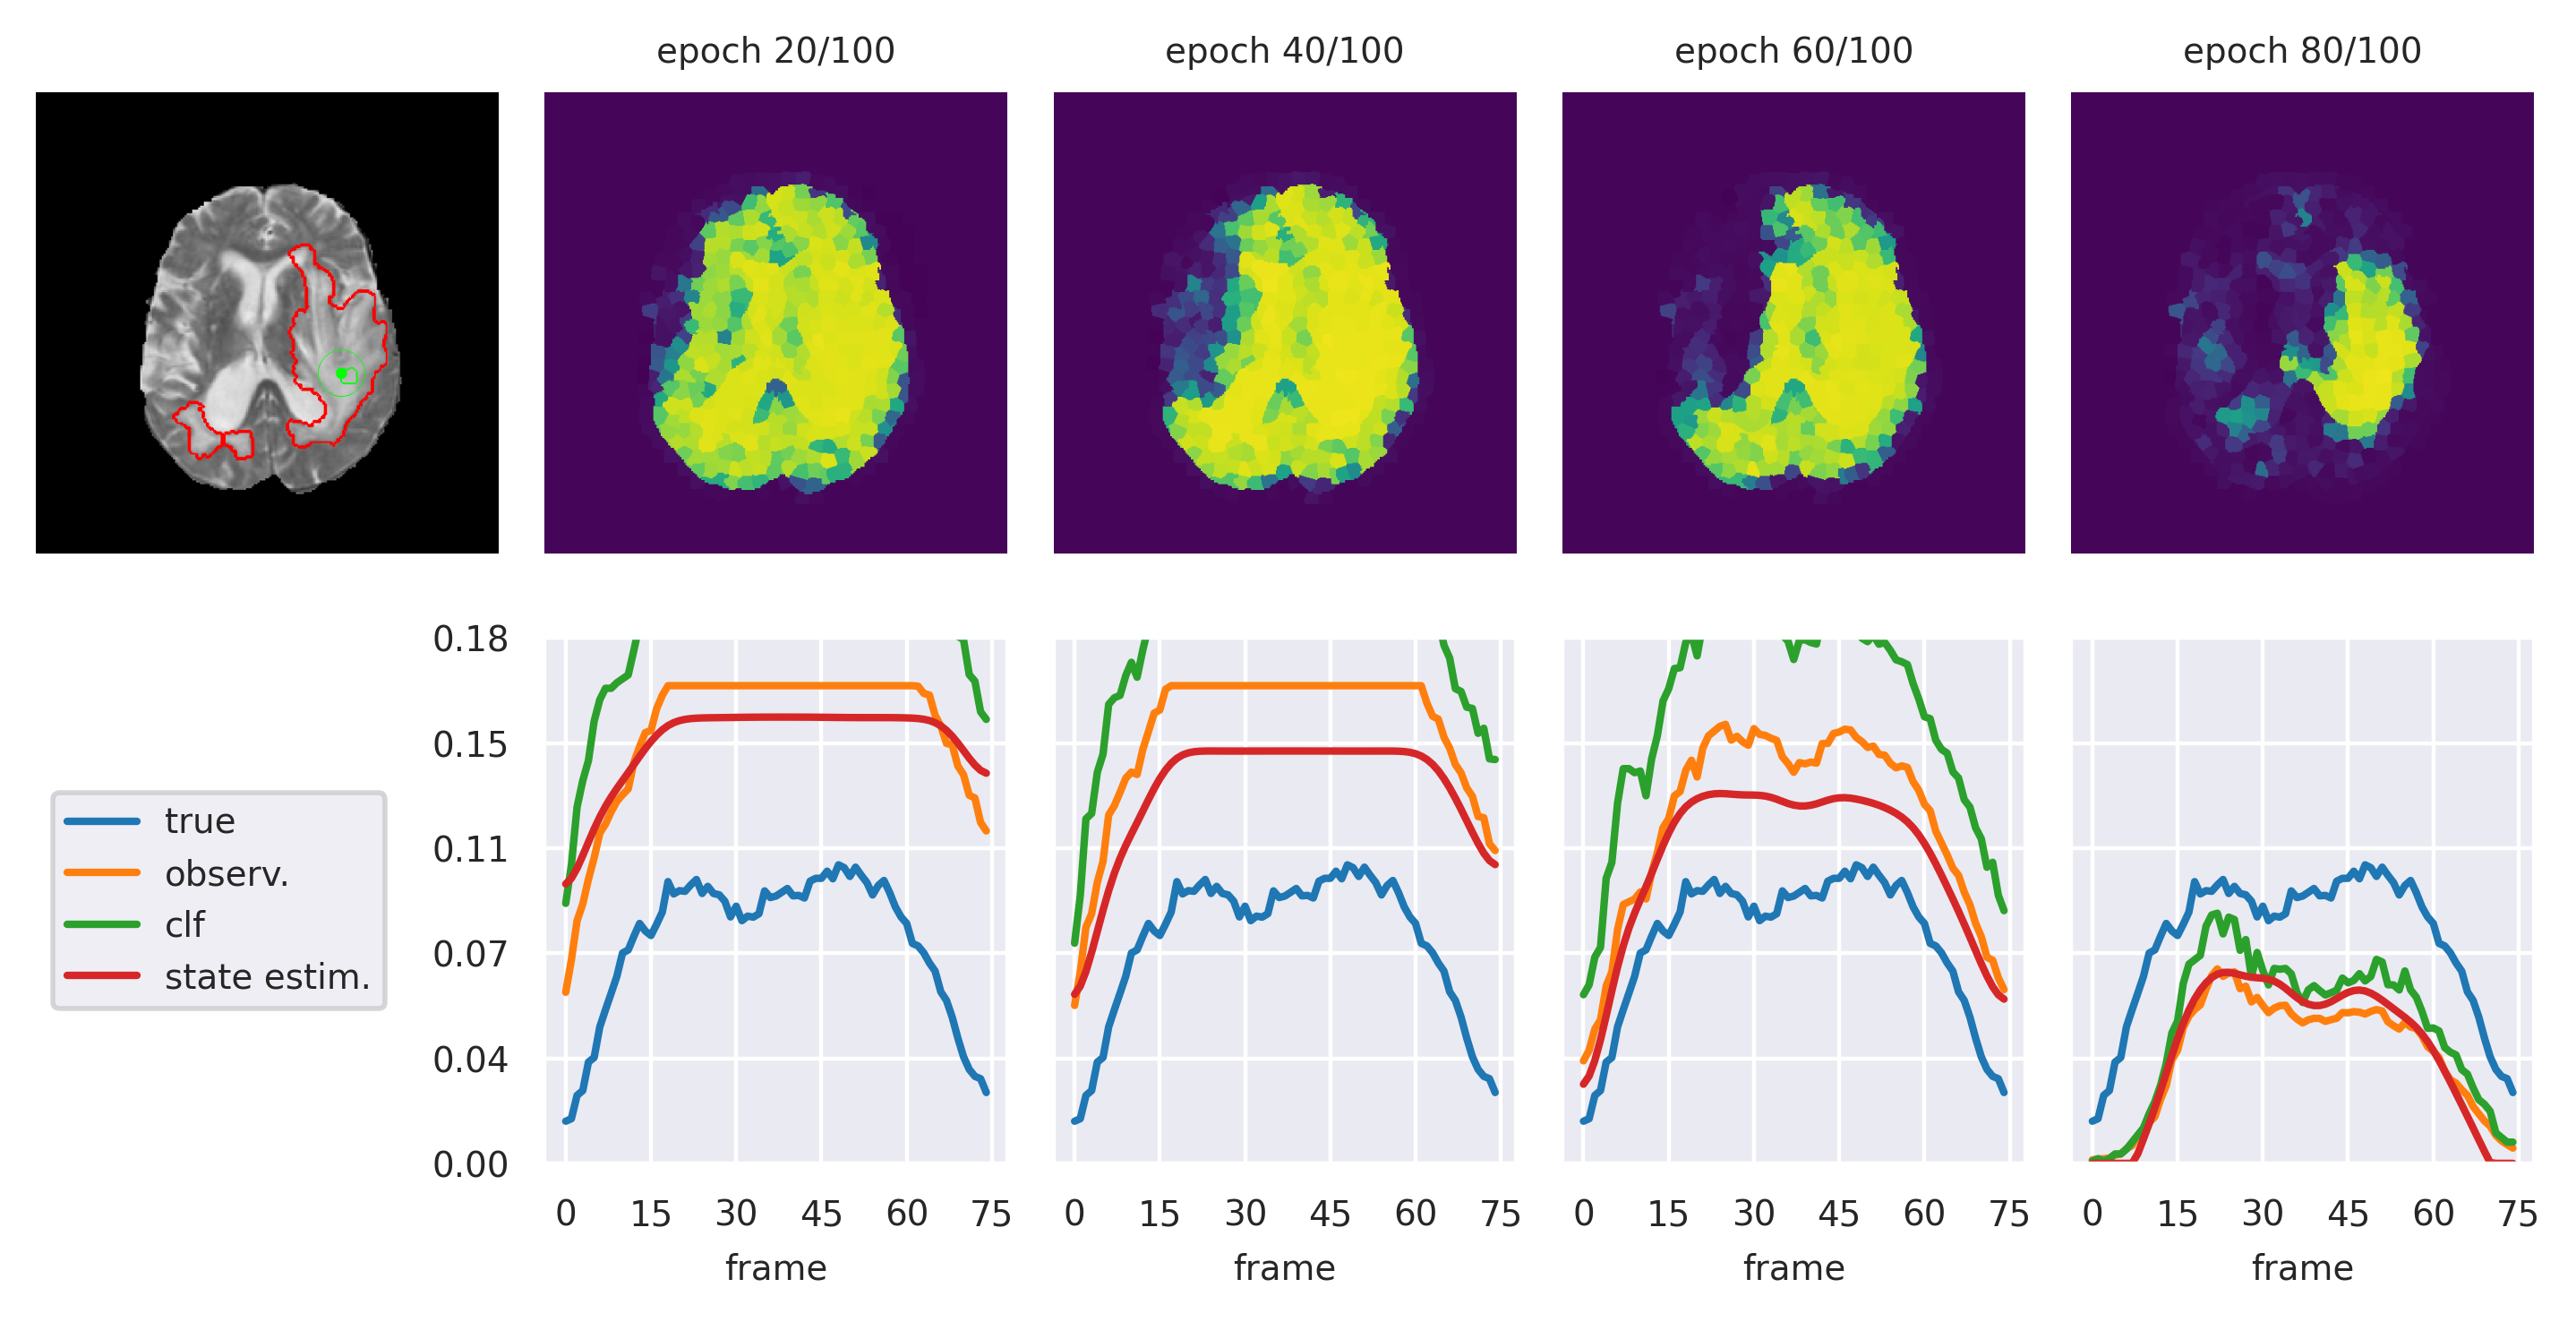
\includegraphics[width=.9\textwidth]{pics/prevs_conv.png}
\label{fig:prevs_conv}
\end{figure*}


%%% Local Variables:
%%% mode: latex
%%% TeX-master: "main"
%%% End:

\subsection{Tracking Framework}
\label{sec:tracking}
In practice, the foreground predictions, as given by the output of our model, are noisy.
As a refinement step, we resort to a similar strategy as \cite{lejeune18}, where the spatio-temporal relations of superpixels are leveraged in a multi-object tracking framework.
We now briefly describe the latter approach, and show where the proposed foreground prediction method fits.


\subsubsection{Tracking as a Linear Program}
\label{sec:orgcf5c794}
Let \(\mathcal{P}=\{x_i\}_{i=1}^{|\mathcal{P}|}\) as a path formed by temporally-ordered superpixels \(x_{i}\), where we omit the time index for conciseness.
The segmentation task reduces to finding an optimal set of paths \(\bm{\mathcal{P}}^*=\{ \mathcal{P}_k\}_{k=1}^K\) so as to minimize a cost.
As further developped in \cite{lejeune18}, the latter problem is first formulated as a maximum a posteriori problem and converted to the integer program:

\begin{multline}
\label{eq:lin_prog}
\bm{\mathcal{P}}^* = \operatorname*{argmin}_{\bm{\mathcal{P}}} \sum_i C_{fg}(i) f_{visit}(i) + \\ \sum_{i,j} C_{trans}(i,j)f_{trans}(i,j) + \sum_{i} C_{in} f_{in}(i)
\label{eq:lin_prog}
\end{multline}

Considered as a network flow problem, the latter integer program is further restricted to edge capacity constraints and flow conservation at the nodes inputs and outputs.

The term $C_{fg}(i)$ defines the cost of selecting superpixel $x_i$ as foreground.
We derive it from the foreground probability of the corresponding superpixel as

\begin{equation}
  \label{eq:cost_fg}
  C_{fg}(i) = -\log \frac{f_\theta(x_i)}{1-f_\theta(x_i)}
\end{equation}

By construction, this relation therefore imposes a negative cost when $f_{\theta}(x) > 0.5$, and a non-negative cost otherwise.
The costs $C_{in}(i)$, express the cost of pushing flow into the network starting from superpixel $x_{i}$.
In particular, for each user-provided 2D location (assumed to be located on the object), we define a circle centered on it of radius $R$.
$C_{in}(i)$ is set to $0$ when the centroid of superpixel $x_i$ is contained within that circle, and $\infty$ otherwise.
The transitions costs $C_{trans}(i,j)$, which define the cost of transiting from $x_i$ to $x_j$, are set to $0$ when $x_i$ and $x_j$ overlap, i.e. have at least $1$ pixel of same location, and $\infty$ otherwise.

To optimize the problem of Eq. \ref{eq:lin_prog}, we resort to the K-Shortest Paths (KSP) algorithm as described in \cite{lejeune18}.

Note that in contrast with \cite{lejeune18}, we simplify the modeling of costs $C_{in}$ and $C_{trans}$.
Also, the latter work performs several iterations of the tracking algorithm by augmenting the set of positives and re-training their foreground model after each iteration.
This augmentation strategy did not prove beneficial in the proposed foreground prediction model.


%%% Local Variables:
%%% mode: latex
%%% TeX-master: "main"
%%% End:

\subsection{Training details, hyper-parameters, and implementation}
We now describe for each component of our pipeline the hyper-parameters and training details.
The code of our foreground prediction model is written in Python using the PyTorch library \cite{paszke19}.
The tracking module is written in C++.
The code of all components is made publicly available \footnote{\url{https://github.com/lejeunel/ksptrack}}.

\subsubsection{Foreground prediction model}
For all our experiments we use a Convolutional Neural Network based on the U-Net architecture \cite{ronneberger15}, as proposed in \cite{ibtehaz20}.
First, in place of simple convolutional layers, we use ``Inception-like'' blocks \cite{szegedy16} to improve robustness to scale variations.
Second, the shortcut connections are replaced by a serie of $3\times3$ convolutional layers with residual connections.
Last, batch normalization layers \cite{ioffe15} are added after each convolutional layer.

For the proposed self-supervised class-prior estimation (Sec. \ref{sec:nnpu} and \ref{sec:pi_estim}), we divide the training into three phases:

\begin{enumerate}
  \item We perform a pre-training phase so as to make our observations more robust.
    In particular, we initialize the weights of our CNN so as to
    make the training focus more on the foreground, as suggested in \cite{lin17}.
    Concretely, we note that the last layer of our decoder is a sigmoid function $\sigma(x)=\frac{1}{1+e^{-x}}$.
    We set the bias of the preceding convolutional layer to $-\log{\frac{1-\pi_{init}}{\pi_{init}}}$, with $\pi_{init}=0.01$.
    All others parameters are initialized using He's method \cite{he15init}.
    The CNN is then trained for $50$ epochs using constant initial prior $\hat \pi_{0}$ following Alg. \ref{alg:sgdnnpu} with a learning rate set to $10^{-4}$.
    \item We optimize the model and class-prior estimates for maximum $100$ epochs as in Alg. \ref{alg:prior_estim} with a learning rate set to $10^{-5}$.
  \item We train using frame-wise priors given by the previous phase for an additional $100$ epochs with a learning rate of $10^{-5}$.
\end{enumerate}

In all phases, we use the Adam optimizer \cite{kingma14} with weight decay $0.01$.
As data augmentation, we use a random combination of additive gaussian noise, bilateral blur, and gamma constrast.

\subsubsection{Recursive Bayesian Estimation}
For the process, transition, and initial covariance matrices, we use diagonal matrices, i.e.
$Q=\sigma_{Q}\mathbb{I}$, $R=\sigma_{R}\mathbb{I}$, and $S=\sigma_{S}\mathbb{I}$, where $\mathbb{I}$ is the identity matrix.
As the observations are often very noisy, we set an observation variance much larger than the process variance, i.e. $\sigma_{Q}=10$ and $\sigma_{R}=0.05$.
$\sigma_{S}$ is set to $0.03$.
The parameters of the control input are set proportional to $\hat \pi_{0}$, i.e. $u_{0}=0.02 \cdot \hat \pi_{0}$, and $u_{T}=0.4 \cdot \hat \pi_{0}$.
For the observation model (Eq. \ref{eq:observ}), we set $\gamma=2$.
The window length of the frame-wise smoothing filter is set proportional to the number of frames: $L=0.05\cdot N$.
The time-period of our stopping condition is set to $T_{s}=10$, and the threshold on the variance is $\tau=0.007$.

\subsubsection{Tracking and superpixelization}
\label{sec:org4560526}
We define for each user-provided 2D location a circle of radius \(R=0.05 \cdot \max\{W,H\}\) centered on the 2D location, where \(W\) and \(H\) are the width and height of frames, respectively.
In order to reduce the number of edges and alleviate the computational requirement, we also prune ``visiting'' edges when their corresponding foreground probability falls below $0.4$.

So as to make the tracking step tracktable, all sequences are pre-segmented into $\sim 1200$ superpixels using SLIC \cite{achanta12}.
Given that our segmentations will be evaluated at pixel-level, the latter pre-processing step induces an upper-bound in accuracy, which we wish to evalute.
To do so, we use the manual ground truth annotation as follows:
Taking as positive the superpixels that overlap the manual ground truth annotations by more than $0.5$ of their area, and the others as negatives, we obtain the optimal superpixel segmentation of our sequence.
We then compare the latter segmentation with the pixel-wise manual ground truth annotation and report the F1-score in Tab. \ref{tab:sp_errors}.

\begin{table}
\centering
\caption{For each type of sequence, we report the maximum F1-score achievable given the early stage superpixel segmentation.}
\label{tab:sp_errors}
\begin{tabular}{lp{1.8cm}}
\toprule
{} &               F1 \\
\midrule
Brain    &  $0.92 \pm 0.02$ \\
Cochlea  &  $0.92 \pm 0.01$ \\
Slitlamp &  $0.92 \pm 0.02$ \\
Tweezer  &  $0.95 \pm 0.01$ \\
\bottomrule
\end{tabular}
\end{table}


%%% Local Variables:
%%% mode: latex
%%% TeX-master: "../../main"
%%% End:



%%% Local Variables:
%%% mode: latex
%%% TeX-master: "main"
%%% End:
